\documentclass{ieeeaccess}
\usepackage{cite}
\usepackage{amsmath,amssymb,amsfonts}
\usepackage{algorithmic}
\usepackage{graphicx}
\usepackage{textcomp}
\usepackage{adjustbox}
\usepackage{rotating}
\usepackage{booktabs}
\usepackage{xcolor}
\usepackage{multirow}
\usepackage{caption}
\usepackage{soul}
\usepackage{url} 
\def\BibTeX{{\rm B\kern-.05em{\sc i\kern-.025em b}\kern-.08em
    T\kern-.1667em\lower.7ex\hbox{E}\kern-.125emX}}
\begin{document}
\history{Date of publication xxxx 00, 0000, date of current version xxxx 00, 0000.}
\doi{10.1109/ACCESS.2017.DOI}

\title{Extreme TinyGPT at the Edge: A Small Language Model to Support Vehicle Manual Interaction}
\author{\uppercase{Thommas K. S. Flores}\authorrefmark{1}, 
\uppercase{João Carlos N. Bittencourt}\authorrefmark{2}, 
\uppercase{Daniel G. Costa}\authorrefmark{3}, \IEEEmembership{Senior Member, IEEE},
and \uppercase{Ivanovitch Silva}\authorrefmark{1}, \IEEEmembership{Senior Member, IEEE}}

\address[1]{Federal University of Rio Grande do Norte/PPgEEC, Av. Senador Salgado Filho, 3000, Lagoa Nova, Natal-Rio Grande do Norte, 59078–970, Brazil, thommas.flores.101@ufrn.edu.br and ivanovitch.silva@ufrn.br}

\address[2]{CETEC, Federal University of Recôncavo da Bahia, Cruz das Almas 44380-000, Brazil; joaocarlos@ufrb.edu.br}

\address[3]{SYSTEC-ARISE, Faculty of Engineering, University of Porto, Porto, 4200-465, Portugal, danielgcosta@fe.up.pt}


\tfootnote{This paper was partly financed by the Brazilian fostering agency CNPq (National Council 503 for Scientific and Technological Development), Process No. 408736/2025-9, and by FCT through the 504 PhD scholarship (2024.02446.BD}



\corresp{Corresponding author: First A. Author (e-mail: author@ boulder.nist.gov).}

\begin{abstract}
Small Language Models (SLMs) can enable privacy-preserving, in-vehicle interactions without dependence on cloud connectivity. However, although discriminative models have been deployed on microcontrollers, generative capabilities still largely depend on high-end edge computers or proprietary Neural Processing Unit-accelerated hardware. To address this gap, this paper introduces the Extreme Tiny Generative Pre-trained Transformer (TinyGPT), a compact framework for offline generative inference on resource-constrained microcontrollers. The proposed workflow uses retrieval-augmented generation (RAG) to synthesize vehicle-manual question-answer pairs offline, which are then used to train a purely parametric MCU-deployable model. At inference time, TinyGPT uses only its trained weights, without a retrieval index, document store, or access to the original manual. The framework also provides a transparent Python-to-C++ conversion pipeline that exports weights as auditable JSON tensors and translates them into self-contained C++ arrays for deterministic floating-point execution. We validate TinyGPT on four MCU platforms, showing that local generative inference is feasible with sub-watt power consumption on the evaluated FPU-enabled devices. The results indicate a trade-off between deployment transparency, energy efficiency, and out-of-distribution question-answering quality for embedded vehicle-manual interaction.
\end{abstract}

\begin{keywords}
TinyML,  Generative AI,  LLM,  Embedded AI, EdgeAI, Smart Vehicle.

\end{keywords}

\titlepgskip=-15pt

\maketitle

 \section{Introduction}

Recent developments in Natural Language Processing (NLP) have led to the adoption of language models on embedded and edge devices \cite{shakhadri2025shakti}, driven by demand for low-latency and privacy-preserving interfaces that operate without continuous cloud connectivity \cite{shakhadri2025shakti}. This evolution has affected several sensor-based application domains, including Smart Cities \cite{theroad}, Industry 4.0 \cite{automotiveSensors}, and the automotive sector \cite{automotiveSensors}. In particular, within the automotive domain, these transformations have enabled new opportunities to integrate embedded assistants that interpret vehicle manuals locally, with potential benefits for driver interaction and safety \cite{electronics13244972}.

In current vehicles, drivers often struggle to find information on maintenance and basic usage. User manuals tend to be dense and hard to navigate, making it hard to find information quickly, particularly in time-sensitive situations. In response, recent research has explored the use of artificial intelligence to improve access to automotive documentation. Examples include natural language question-answering systems that retrieve information directly from vehicle manuals \cite{park2024maqa}, as well as chatbot-based solutions powered by Large Language Models (LLMs) that enable conversational interaction with automotive manuals \cite{lee2023llmchatbot}. Despite these advances, several limitations remain. Many existing approaches depend on cloud connectivity or external services, which can introduce latency, reduce availability in areas with limited or no network coverage, and compromise reliability in real-world driving conditions. Furthermore, this reliance on remote processing raises concerns about data privacy and security, as modern vehicles generate volumes of personal and operational data that may be exposed during transmission or storage on third-party servers \cite{yang2024privacy,he2025securitysurvey}. These constraints highlight remaining challenges in providing privacy-aware access to vehicle information within connected automotive ecosystems.

Recently, LLMs have been considered a potential means to optimize the querying and retrieval of vehicular data for non-specialist users. To that end, embedding these models in affordable, small electronic units has been explored, potentially bridging the gap between efficiency and practicality, with research in ``AI on the edge`` gaining attention \cite{iiot}. However, deploying language models on Microcontroller Units (MCUs) is constrained by limited memory, processing power, and energy availability \cite{wu2021tiny}. LLMs remain impractical for such environments because of their computational cost and memory footprint \cite{strubell2019energy}. In contrast, Small Language Models (SLMs) provide a balance between performance and efficiency, enabling natural language capabilities on constrained hardware.

Recent research has also addressed this area by optimizing inference engines and model architectures. EdgeMoE, for instance, introduced a sparse Mixture-of-Experts (MoE) model adapted to hierarchical memory, reducing I/O overhead and memory use~\cite{yi2025edgemoe}. This approach enables selective activation of experts, thereby lowering computational cost. Empirical evaluations of SLMs such as TinyLlama, Phi-3, and LLaMA-3 have shown that latency, memory usage, and power consumption depend on the target hardware~\cite{islam2024characterizing, qin2025empirical}.
%
Other frameworks, such as TinyLLM, have enabled the training and deployment of compact models for specific tasks, achieving reported token generation rates with task-level accuracy~\cite{10.1145/3636534.3697466}. Similarly, the Deeploy compiler generates optimized C code for heterogeneous hardware architectures, enabling efficient inference of TinyStories-based models on RISC-V MCUs using only on-chip memory~\cite{scherer2024deeploy}. Although these approaches have shown progress, they often rely on toolchains, optimizations, or quantization strategies, which can reduce inspectability in safety-aware domains. In this paper, transparency denotes inspectable code and deterministic numerical execution, while factual correctness is evaluated separately through task-level metrics.


In this context, we introduce Extreme TinyGPT, a compact GPT-based small language model (SLM) designed for offline deployment on affordable microcontrollers with inspectable implementation. The approach uses offline RAG to synthesize a training and testing dataset from the manual, after which the deployed model operates solely from its learned parameters. This positioning treats the model as a closed-domain parametric memory that compresses selected vehicle-manual knowledge into FP32 weights. To validate the architecture, we evaluate a text-to-text application in which user queries are mapped to generated responses and compare behavior across training and test subsets. The proposed methodology includes a direct Python-to-C++ conversion pipeline that eliminates external dependencies while preserving floating-point equivalence between training and deployment. We validate the approach on four MCU platforms (Arduino Nano BLE Sense 33, Portenta H7, ESP32, and Raspberry Pi Pico), showing deterministic execution and device-dependent resource utilization, with lower latency on FPU-equipped MCUs.




The organization of this article is as follows. Section~\ref{sec:related_works} reviews related work. Section~\ref{sec:method} outlines the proposed methodology and conversion workflow. Section~\ref{sec:exp_setup} describes the experimental instrumentation and setup. Section~\ref{sec:results} presents a discussion of the results, and Section~\ref{sec:conclusion} concludes the study, offering insights into potential future research.



\section{Related Work}\label{sec:related_works}

The migration of language models to edge devices is driven by the need for low-latency, privacy-preserving, and cloud-independent inference. Research in this domain has mainly followed two directions: the design of compact SLM architectures and the development of deployment toolchains for resource-constrained hardware.

Significant progress has been documented on the design of inherently efficient model architectures. Prominent examples, such as TinyLlama \cite{zhang2024tinyllama} and MobileLLM \cite{mobilellm2024}, demonstrate that deliberate architectural choices favoring deep-yet-thin structures can yield exceptional performance-per-parameter ratios well-suited to mobile scenarios. However, under the extreme constraints of microcontrollers, further compression is mandatory. Works including TinyFormer \cite{yang2023tinyformer} and MCUBERT \cite{10.1145/3676536.3676747} demonstrate the efficacy of aggressive quantization and neural architecture search to reduce model footprints to sub-megabyte scales. More recent innovations, such as the Fused-Weight Self-Attention mechanism \cite{JungOptimizing2025}, go beyond compression by directly re-engineering the transformer block to mitigate memory bottlenecks inherent to MCU architectures.

Complementing these architectural innovations, a parallel body of work addresses the full-stack deployment pipeline. Frameworks such as Deeploy \cite{scherer2024deeploy} and MCUFormer \cite{liang2023mcuformer} provide systems that incorporate memory-aware scheduling, kernel optimization, and compiler techniques tuned to harness heterogeneous cores and Neural Processing Units. These solutions have been validated primarily on research-oriented platforms such as the GAP9 SoC \cite{BusiaTinyTransformer2025} and custom RISC-V chips equipped with dedicated accelerators \cite{scherer2024deeploy}.

Concurrently, research has expanded into domain-specific applications, validating the utility of generative AI in embedded environments. \cite{varshni2025embedded} investigated embedded LLMs to enhance automotive Human-Machine Interfaces (HMI), while \cite{yauri2024generative} integrated generative models into IoT devices for voice assistance. However, these application-centric studies typically rely on single-board computers (SBCs) or Linux-based gateways to manage computational overhead, distinguishing them from the bare-metal microcontroller constraints addressed in this work. Table~\ref{tab:related_work} compares the main contributions related to model efficiency and deployment strategies.

Despite these advancements, current approaches leave a deployment gap. Many efficiency-oriented frameworks remain coupled to specialized toolchains, quantization pipelines, or hardware accelerators, which can complicate reproducibility, debugging, and independent inspection. In automotive and other safety-aware domains, inspectable implementation and predictable execution are useful conditions for engineering assessment, while factual reliability must still be evaluated at the task level. In addition, many evaluations focus on a limited set of high-performance platforms, leaving the behavior of generative language models across affordable general-purpose microcontrollers insufficiently characterized.



To address this gap, the present study introduces Extreme TinyGPT, a compact GPT-based SLM coupled with a streamlined Python-to-C++ conversion pipeline for offline, dependency-free deployment. The contribution is methodological and engineering-oriented: offline RAG and LLM-generated data are used to compress selected vehicle-manual knowledge into a small parametric model, and the deployed MCU system then operates without a retrieval index, document store, or access to the original manual. The methodology preserves floating-point equivalence between training and inference and is evaluated on four commercially available MCU platforms, showing that autoregressive text generation can be executed on accessible microcontrollers. Unlike deployment pipelines such as TFLite Micro~\cite{https://doi.org/10.1002/er.7713} and EdgeImpulse~\cite{s22145174}, which rely on interpreter runtimes or quantization schemes, the proposed pipeline generates human-readable C++ code with no external runtime dependencies while maintaining 32-bit floating-point determinism. This property supports software inspection and reproducibility, while factual and safety-oriented behavior are evaluated at the task level.





\begin{table*}[htbp]
\scriptsize
\centering
\caption{Comparative Analysis of SLMs and Their Deployment on Edge Devices.\label{tab:related_work}}
\begin{adjustbox}{max width=0.95\paperheight}
\begin{tabular}{@{}p{2cm}p{2cm}p{3cm}p{2.5cm}p{2.9cm}@{}}
\toprule
\textbf{Reference} & \textbf{Model} & \textbf{Optimization} & \textbf{Application} & \textbf{Hardware} \\
\midrule
\cite{yang2023tinyformer} & TinyTransformer & Int8 quantization, optimized attention kernels & Gesture recognition & STM32, GAP8 \\\\
\cite{10.1145/3676536.3676747} & BERT-mini & Low-rank approximation, NAS & Text classification & Generic MCUs \\\\
\cite{liang2023mcuformer} & MCUFormer  & One-shot NAS, memory-aware scheduling & Visual recognition & STM32 MCUs \\\\
\cite{scherer2024deeploy} & TinyStories-class & Int8 quantization, KV caching, NPU compiler & Autoregressive text generation & Siracusa MCU (RISC-V NPU) \\\\
\cite{JungOptimizing2025} & Encoder-only Transformers & Fused-weight self-attention, depth-first tiling & General TinyML tasks & STM32H7, GAP9 \\\\
\cite{BusiaTinyTransformer2025} & Tiny Transformer & 8-bit quantization, parallel execution & ECG classification & GAP9 MCU \\\\
\cite{zhang2024tinyllama} & TinyLlama & Architectural efficiency, scaled pretraining & General language tasks & (Design-focused) \\\\
\cite{mobilellm2024} & MobileLLM & Shared expertise, dense scaling law & General language tasks & Mobile/Edge GPUs \\\\
\cite{CaoEmbedAgent} & DeepSeek-R1, Claude 3.7 & RAG, compiler feedback (Tool-use) & Embedded code generation & Raspberry Pi Pico, ESP32 \\\\
\cite{edgeLM2024} & EdgeLM & Selective execution, hybrid quantization & On-device assistants & Snapdragon, Jetson \\\\
\cite{varshni2025embedded} & Quantized LLMs & Context-aware processing & Automotive HMI & Edge Computers \\\\
\cite{yauri2024generative} & Generative LM & Integration with IoT peripherals & Voice Assistant & IoT Single Board Computers \\\\

\textbf{Our Proposal} & Extreme TinyGPT & Float32 preservation, Python-to-C++ transpilation, dependency-free runtime & Offline embedded in-vehicle Q\&A using a parametric SLM without retrieval & Arduino Nano 33 BLE, Portenta H7, ESP32, RPi Pico \\
\bottomrule
\end{tabular}
\end{adjustbox}
\end{table*}


\section{Methodology}\label{sec:method}

The development of compact language models for in-vehicle assistance has become increasingly relevant as modern vehicles require more intuitive access to technical information under strict computational and connectivity constraints. In this section, we present the methodology for deploying a small language model on microcontroller units as illustrated in Figure~\ref{fig:pipeline}. The pipeline covers all stages, from acquiring vehicle manuals and extracting knowledge to preprocessing, model training, and final deployment on embedded hardware. 

\begin{figure*}[htpb]
\centering
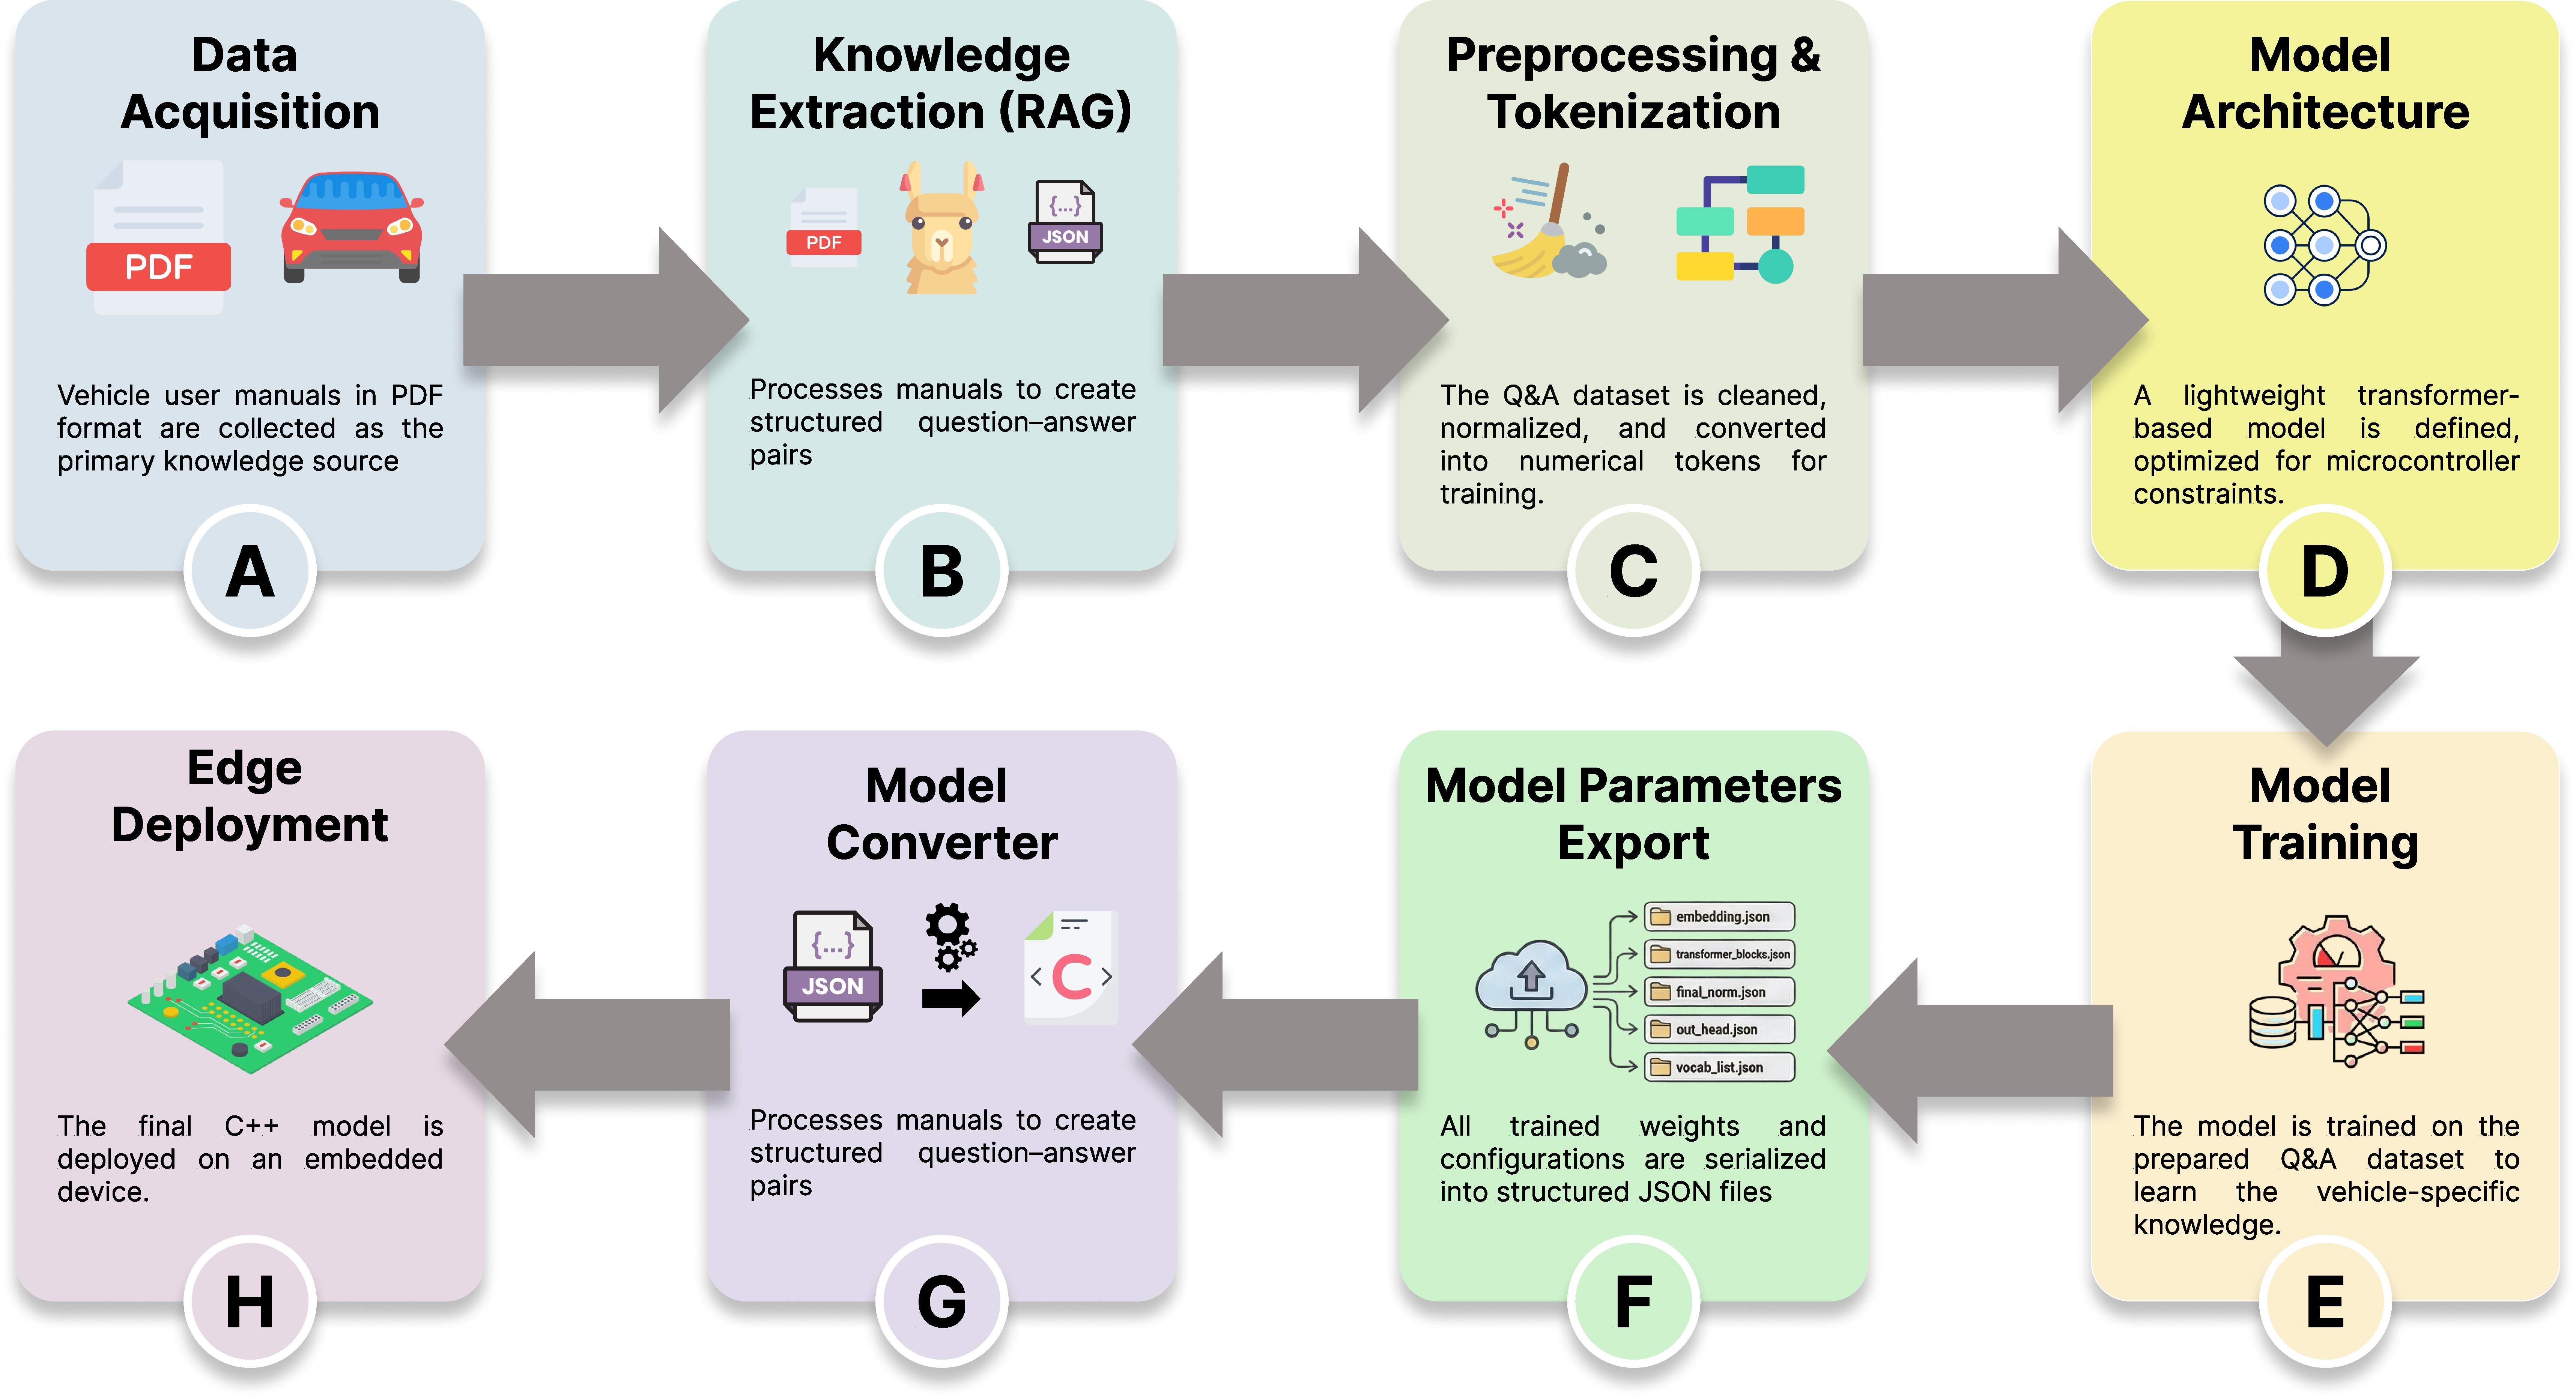
\includegraphics[width=0.85\linewidth]{Figures/pipeline.pdf}
\caption{Workflow from vehicle data acquisition and knowledge extraction to model training, C++ conversion, and deployment on embedded hardware.}
\label{fig:pipeline}
\end{figure*}

A key novelty of this workflow is concentrated in stages (F)–(H), where the model trained in a high-level Python environment is automatically exported, converted into a compact C++ representation, and deployed on resource-constrained devices. This design enables fully on-device inference while preserving the structural integrity of the trained model, thereby supporting practical deployment under strict memory, energy, and connectivity constraints.

\subsection{Data Acquisition}

The data used in this work were obtained from manufacturers' official vehicle user manuals in PDF format. These manuals served as the primary source of knowledge and were segmented into fragments of up to 100 characters. This empirical limit was chosen through a supervised analysis to balance contextual preservation with the model's limited context window.

\subsection{Knowledge Extraction}
\label{sec:knowledge_extraction}

The dataset was synthesized through a pipeline that transforms raw manual text into a structured instruction-following format. First, textual content was extracted from PDF technical manuals, a format commonly used for documents with complex layouts and graphical elements.

After extraction, the text was segmented into semantically coherent chunks. Instead of applying a fixed-length character split, the algorithm preserved natural paragraph boundaries. Consecutive paragraphs were grouped until a predefined token threshold was reached, at which point a new chunk began. This strategy helps each chunk retain a self-contained idea or procedural description while balancing contextual integrity with computational practicality for model training.

Finally, each chunk was converted into a question-answer pair using a Retrieval-Augmented Generation (RAG) system built on LLaMA~3.2~\cite{llama3} and executed in a strictly local, offline environment. This step served only to generate a synthetic dataset of 1,000 Q\&A pairs. The RAG system retrieved relevant manual chunks to produce factually grounded questions and answers; after dataset creation, however, the RAG pipeline was discarded. The assistant model deployed on the MCU is a standard autoregressive transformer trained on this synthetic data. During inference, it has no access to a retrieval index, document store, or the original manual; all answers are generated solely from its learned parameters.

The resulting instruction-response pairs were stored in JSONL format to support fine-tuning and reproducibility. The final dataset consists of compact, domain-specific knowledge units derived from the original manual. Representative examples are shown in Table~\ref{tab:qa_examples}.



\begin{table*}[!t]
\small
\centering
\caption{Representative instruction-response pairs generated from the vehicle manual.}
\label{tab:qa_examples}

\begin{tabular*}{\textwidth}
{@{\extracolsep\fill}p{7cm} p{6cm}}
\toprule
\textbf{Instruction (Question)} & \textbf{Response (Answer)} \\
\midrule
What does the symbol DANGER represent? & Warning or threat indicator \\
What is under the Volkswagen badge? & Radar sensor for assist systems \\
What are the first two parts of a car? & Engine compartment and windscreen \\
Where is the rain and light sensor located? & Near the interior mirror \\
What features are included in this vehicle? & Sensors for assist and jacking points \\
\bottomrule
\end{tabular*}
\end{table*}






\subsection{Preprocessing, Curation, and Tokenization}

Prior to model training, the Q\&A dataset underwent a systematic curation process to ensure data quality, consistency, and relevance. This stage involved the removal of duplicated samples, incomplete or ill-formed question–answer pairs, and entries with semantic misalignment between questions and corresponding answers. Additionally, samples exhibiting excessive noise, formatting artifacts, or domain-irrelevant content were excluded to reduce bias and improve learning stability.

Following curation, each remaining Q\&A pair underwent a cleaning and normalization pipeline that removed redundant symbols, standardized punctuation, and unified text casing and formatting. Tokenization then transformed the processed textual sequences into numerical tokens suitable for model training. Special control tokens (\texttt{<pad>}, \texttt{<sos>}, \texttt{<eos>}, \texttt{<unk>}, and \texttt{<sep>}) were employed to explicitly encode sequence boundaries, padding, unknown terms, and the separation between questions and answers.


\subsection{Model Architecture}

The proposed model, Extreme TinyGPT, utilizes a Decoder-only Transformer architecture. Unlike encoder-based models (e.g., BERT) which utilize bidirectional attention, our model employs masked multi-head causal attention. This masking ensures that the attention mechanism for position $t$ can only attend to positions $\le t$, preserving the autoregressive property required for next-token generation. Although the individual transformer blocks share structural similarities with standard encoders (Feed-Forward Networks and Normalization), the causal masking strictly defines the model as a generative decoder. As shown in Figure~\ref{fig:model_architecture}, the architecture comprises token embeddings, positional encodings, multiple transformer blocks, and a final linear projection layer. Each transformer block includes Layer Normalization, masked multi-head causal attention, residual connections, and a feed-forward network with a Gaussian Error Linear Unit (GeLU) activation. This configuration enables fine-grained hyperparameter tuning, such as the number of attention heads and transformer depth, to match different hardware capabilities.


The causal masking in the multi-head attention mechanism enables autoregressive next-token prediction, allowing iterative text generation despite the encoder-like block structure. This architecture supports output sequences up to the 32-token context length through sequential token appending during inference.




The proposed model, named Extreme TinyGPT, is a decoder-only transformer with causal self-attention, intended for deployment on microcontroller-class devices. As illustrated in Figure~\ref{fig:model_architecture}, the architecture consists of token embeddings, positional encodings, multiple transformer blocks, and a final linear projection layer. Each transformer block comprises Layer Normalization, masked multi-head causal attention, residual connections, and a feed-forward network with Gaussian Error Linear Unit (GeLU) activation. The causal attention mechanism prevents tokens from attending to future positions in the input sequence.


Causal masking enables autoregressive next-token prediction and allows the model to generate sequences up to the 32-token context window through sequential token appending. During inference, the model predicts one token per step and appends the prediction to the input sequence for subsequent forward passes. This inference procedure corresponds to the decoder-only transformer architecture commonly adopted in GPT-style models. In contrast to bidirectional encoder architectures such as BERT, which produce fixed-length representations for classification tasks, the proposed decoder architecture supports autoregressive text generation without relying on separate encoder and decoder stacks.






\begin{figure}[htpb]
\centering
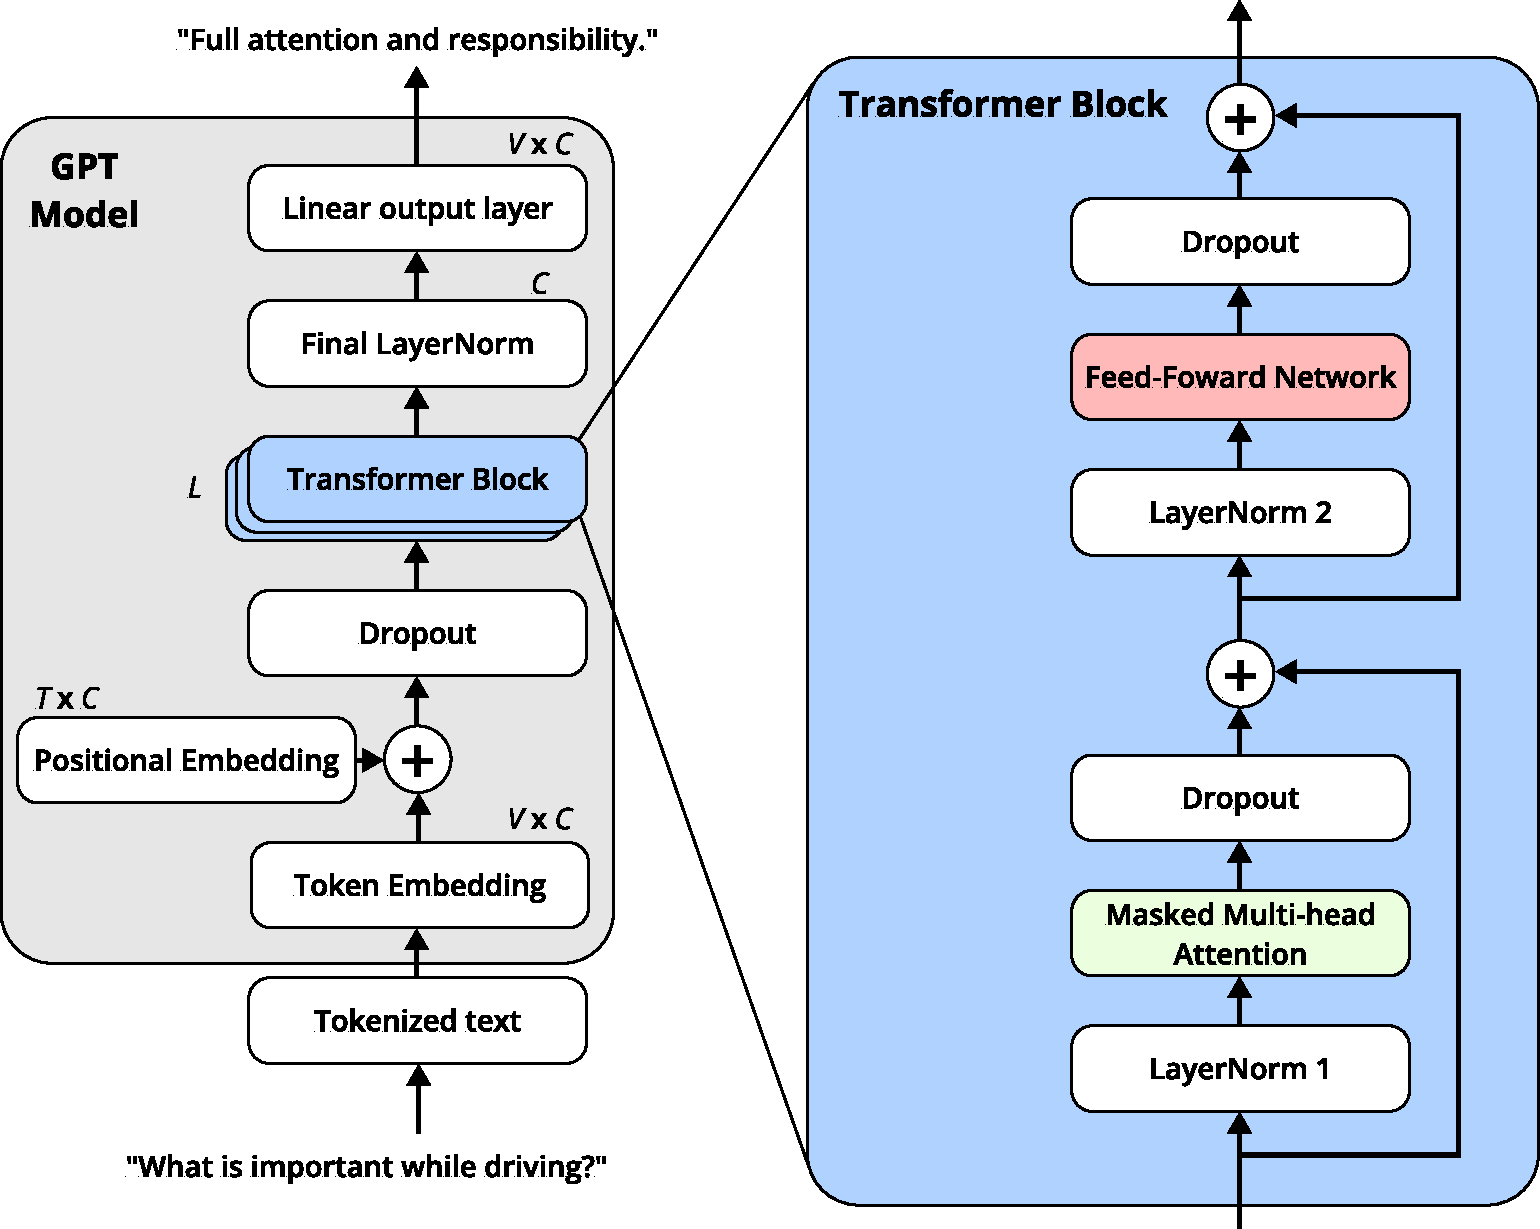
\includegraphics[width=0.8\linewidth]{Figures/transformer.pdf}
\caption{Overview of the TinyGPT architecture, showing the processing flow from tokenization to response generation. The right panel depicts the internal structure of the Transformer Block used during autoregressive inference. The matrices $V \times C$ and $T \times C$ denote the token embedding table (vocabulary size $\times$ embedding dimension) and the sequence embeddings (number of tokens $\times$ embedding dimension), respectively.}
\label{fig:model_architecture}
\end{figure}

\subsection{Model Training}

The models were trained with the Adam optimizer on a 700-sample training set derived from the 1,000 question-answer pairs generated offline by the RAG pipeline, with the remaining 300 samples used for testing (Subsection~\ref{sec:knowledge_extraction}). We evaluated architectures with embedding dimensions $d_{model} \in \{12, 16, 20, 24\}$, attention heads $h \in \{1, 2, 3, 4\}$, and transformer layers $L \in \{1, 2, 3, 4\}$. All models used a vocabulary of 445 tokens and a context length of 32 tokens.

\subsection{Model Parameters Export}

Upon completion of the training phase, the entire set of model parameters is systematically serialized and exported to structured JSON files. This step is orchestrated by computational routines that meet the precision requirements and support the quantization strategies necessary for efficient deployment.

The extraction procedure, performed by our toolchain, yields a set of files that collectively define the trained model's state:

\begin{itemize}
    \item \textbf{config.json}: defines the core hyperparameters and architectural configuration, specifying structural parameters such as the total number of attention heads, the model depth in terms of transformer layers, the embedding dimensionality, and the overall vocabulary size.

    \item \textbf{vocab\_list.json}: enumerates the vocabulary as a sequence of string tokens, effectively defining the linguistic domain understood by the model.

    \item \textbf{embedding.json}: stores the weight tensors for the initial processing stages, specifically the data required for both the token representations and the positional encoding layers.

    \item \textbf{transformer\_blocks.json}: encapsulates the complete parameter set for each layer of the architecture, including all weights and biases inherent to the multi-head attention mechanisms and the feed-forward network components.

    \item \textbf{final\_norm.json}: preserves the scaling and shifting parameters required for the layer normalization operation, which is applied immediately after the final transformer block to stabilize the output.

    \item \textbf{out\_head.json}: contains the weight matrix for the final linear projection layer, which maps the internal representations back to the vocabulary space to generate predictions.
\end{itemize}



\subsection{Model Converter}

The code generation phase serves as the pivotal bridge between the high-level training environment and the low-level embedded deployment, automatically translating the SLM parameters into optimized C++ source code tailored for microcontroller execution. This stage transforms abstract mathematical weights into a concrete implementation suitable for running on hardware with limited computational resources.

The process begins by ingesting the structured files exported during the training phase, which contain the model embeddings, transformer weights, normalization parameters, and configuration metadata. Upon loading, these artifacts undergo a rigorous validation procedure to ensure internal consistency and completeness. After validation, the system reconstructs the vocabulary and extracts core architectural definitions, such as the total number of layers, the number of attention heads, and the embedding space dimensions. Simultaneously, special control tokens that define sequence boundaries are identified and mapped to their corresponding numerical identifiers, preserving the logical flow of text generation.

A dedicated Python-based generator converts these validated artifacts into two primary C++ source files: a header file and an implementation file. This tool systematically converts the model parameters into static C++ arrays representing weights, biases, and normalization constants. These arrays are formatted with standard floating-point precision to maximize numerical accuracy and fidelity to the original trained model. This direct representation allows the embedded system to replicate the behavior of the high-level model without requiring compression artifacts or approximation schemes.

The generated implementation file encapsulates the mathematical routines required for inference, including matrix-vector multiplication, layer normalization, activation functions, and probability computation. The complete transformer architecture, comprising multi-head attention mechanisms, feed-forward networks, and residual connections, is reconstructed directly in C++. This direct translation ensures that the embedded execution remains deterministic and strictly consistent with the behavior observed in the original Python-based research environment.

Complementing the logic, the accompanying header file defines architectural constants and declares the generated arrays and function prototypes. To support compatibility across different microcontroller architectures, the code uses conditional compilation directives and strategic memory allocation techniques. This approach places large data arrays in non-volatile flash memory rather than Random Access Memory (RAM), supporting deployment across platforms, from simple Advanced Virtual RISC (AVR) chips to ARM-based processors, without relying on external inference libraries.

In its final assembly, the generator constructs a forward inference function that computes output probabilities for token prediction, as well as routines for sequence generation and decoding. The result is a self-contained, C++ project that reproduces the language model's inference pipeline, enabling specialized edge computing applications on minimal hardware.


\subsection{Edge Deployment and Inference}


The deployment strategy adopts a self-contained, hardware-oriented approach, enabling SLMs to run autonomously on MCUs. The entire architecture is encapsulated in a unified set of source files that contain the inference logic, pre-trained weights, and static memory buffers. This integration defines architectural constants such as vocabulary size, embedding dimensionality, layer count, and context length, as well as tensor and auxiliary array declarations. To conserve limited RAM, these data structures are explicitly placed in non-volatile flash memory. The implementation provides the mathematical routines required for attention mechanisms, normalization, and activation functions, allowing the model to execute without external dependencies or runtime frameworks. This design supports deterministic behavior, inspectable computation, and offline operation in resource-constrained edge environments, while factual correctness remains an empirical property evaluated separately.

At runtime, the inference cycle begins by ingesting user input as a text string. The raw text is tokenized into integer identifiers using the embedded vocabulary functions defined in the header files. Each token is mapped to its corresponding index in the model’s internal vocabulary array. Subsequently, the resulting integer sequence is adjusted to match the predefined context window size through truncation or padding, ensuring compatibility with the model’s fixed input requirements.

The inference pipeline proceeds through a series of computational stages that replicate the transformer architecture. Initially, each token identifier is transformed into a dense vector by summing its semantic embedding with the corresponding positional encoding. This produces a matrix that captures both the token identity and the sequential order of the input. These representations are then processed through a stack of transformer blocks, each comprising a multi-head attention mechanism and a feed-forward network. Within each attention block, the query, key, and value matrices are computed, and a scaled dot-product operation is applied with causal masking to preserve the model's autoregressive property. The outputs are projected linearly, combined with the original input via residual connections, and then normalized. The feed-forward network applies linear transformations separated by activation functions, mirroring the structural configuration used during training.

After the transformer layers are complete, the resulting hidden representation undergoes a final normalization step using stored scaling and shifting parameters. This normalized vector is then multiplied by the output projection matrix to produce logits over the entire vocabulary, effectively representing the predicted probability distribution for the next token in the sequence.

The text generation process is performed iteratively through an autoregressive loop. The model selects the most probable token using a greedy decoding strategy, appends it to the existing sequence, and repeats the inference cycle until a specific end-of-sequence token is produced or a predefined generation limit is reached. The decoded output is reconstructed into readable text using the embedded mapping functions, enabling the display or transmission of the generated response. For interactive tasks such as question answering, an internal routine handles both token prediction and string reconstruction while controlling the use of memory buffers.

Contrary to standard encoder-only architectures that produce fixed-length outputs limited to input length, our causal transformer enables autoregressive generation. During inference, the model processes the current context window once per transformer block to predict the next token, which is then appended to the input sequence. This iterative process continues until an end-of-sequence token is generated or the maximum generation length is reached, supporting outputs that match or are shorter than the 32-token context window without fixed input-output length restrictions. This capability was empirically validated on vehicle manual Q\&A tasks.

In the final integration stage, the compiled firmware is integrated into the microcontroller environment. The main control script initializes hardware peripherals, loads model data from flash memory, and manages serial communication channels for user interaction. The inference task runs entirely on-device, relying solely on embedded parameters and statically allocated buffers. This deployment methodology demonstrates the feasibility of running compact transformer-based language models on MCUs in fully offline edge-computing scenarios. Real-time behavior, however, is platform-dependent and is supported only on the faster FPU-enabled devices evaluated in this study, not uniformly across all tested MCUs.


\section{Proposed Evaluation Scenario}
\label{sec:exp_setup}

The evaluation aims to address the following research questions:

\begin{enumerate}
\item \textbf{RQ1:} How does the architectural variation of SLMs, in terms of the number of layers and attention heads, influence training accuracy and efficiency, as measured by metrics such as training time, loss, and parameter complexity?

\item \textbf{RQ2:} What are the effects of deploying SLMs across different MCUs in terms of inference time, energy consumption, and platform-dependent suitability for interactive automotive applications?
\end{enumerate}

The scripts and libraries are publicly available on GitHub \cite{tinygpt}, enabling researchers and practitioners to replicate and extend this work.





\subsection{Instrumentation}

The training process was conducted on a high-performance personal computer with a 12th Gen Intel Core i5-8265U processor (1.60 GHz), 32 GB of RAM, and Windows 11 Home (version 24H2).

To evaluate the effectiveness of the proposed approach and validate its performance in embedded environments, four MCU units were selected: the Arduino Portenta H7 (STM32H747, Dual-Core Arm\textregistered  Cortex\textregistered-M7/M4), ESP-WROOM-32 DEVKit V1 (Xtensa\textregistered Dual-Core 32-bit LX6), Raspberry Pi Pico (ARM Cortex\textregistered-M0+ Dual-Core), and Arduino Nano 33 BLE Sense (Arm\textregistered Cortex\textregistered-M4F with Floating Point Unit (FPU)). Their technical specifications are listed in Table~\ref{tab:microcontrollers}. Inference time was measured as the wall-clock duration from the start of the forward pass until the end-of-sequence token was generated or the maximum generation length was reached, captured via hardware timer on each board. Energy consumption was estimated by multiplying the measured supply current (obtained with a series ammeter on the power rail) by the supply voltage and the measured inference duration. All measurements were repeated five times per configuration, and the reported values are the arithmetic mean.

\begin{table}[htpb]
\begin{center}
\caption{Considered MCUs for the experiments.}
\label{tab:microcontrollers}
\begin{tabular}{l c c c} 
\toprule
\multicolumn{1}{c}{\textbf{Development board}} &
\multicolumn{1}{c}{\textbf{Clock Speed}} &
\multicolumn{1}{c}{\textbf{RAM}} &
\multicolumn{1}{c}{\textbf{Flash}} \\
\midrule
Arduino Portenta H7           & 480 MHz               & 1 MB + 8 MB    & 16 MB    \\  
Arduino ESP32                & 240 MHz               & 520 KB         & 4 MB    \\ 
Raspberry Pi Pico             & 133 MHz               & 264 KB         & 2 MB    \\
Arduino Nano 33 BLE S.      & 64 MHz                & 256 KB         & 1 MB    \\ 
\bottomrule
\end{tabular}
\end{center}
\end{table}

\subsection{Evaluation Metrics}
\label{subsec:eval_metrics}

To ensure a holistic assessment of the proposed SLM, we adopt a two-stage evaluation framework. This approach captures both the models' theoretical linguistic capabilities and their practical feasibility when deployed on resource-constrained hardware.

During training and evaluation, we monitor optimization performance, linguistic quality, semantic similarity, factual consistency, safety, and computational cost. The following metrics are considered:

\begin{itemize}
    \item \textbf{Cross-Entropy Loss and Perplexity:} Cross-Entropy Loss is adopted as the optimization objective during training, while Perplexity measures the model's uncertainty when predicting the next token. Lower perplexity values indicate a better representation of the underlying language distribution.

    \item \textbf{Linguistic Precision (Accuracy and Exact Match):} Token Accuracy measures the proportion of correctly predicted tokens, whereas Exact Match evaluates whether the entire generated sequence exactly matches the reference sequence, providing a stricter assessment of generation quality.

    \item \textbf{Semantic Similarity (BLEU):} The BLEU score evaluates the lexical and semantic similarity between generated and reference texts by measuring the overlap of $n$-grams. Higher BLEU values indicate greater agreement with the expected output.

    \item \textbf{Factual Correctness (FC):} This metric estimates the proportion of generated responses that are sufficiently consistent with the reference answer. A response is considered factually correct when its sentence-level semantic similarity exceeds a predefined threshold. The Factual Correctness Rate is computed as:
    \begin{equation}
    \text{FC} = \frac{1}{N}\sum_{i=1}^{N}\mathbf{1}\!\left[\text{BLEU}(\hat{y}_i,y_i)\geq0.5\right],
    \end{equation}
    where $\hat{y}_i$ and $y_i$ denote the generated and reference responses, respectively.

    \item \textbf{Manual Grounding Score (MG):} The Manual Grounding Score quantifies how closely the generated response is aligned with the reference text using the ROUGE-L F-measure, which evaluates the longest common subsequence between both sequences:
    \begin{equation}
    \text{MG}=\text{ROUGE-L}(\hat{y}_i,y_i).
    \end{equation}
    Higher values indicate greater lexical overlap with the reference content.

    \item \textbf{Hallucination Rate (HR):} Hallucination Rate measures the proportion of generated tokens that are not supported by the reference answer. It is defined as one minus the token-level precision:
    \begin{equation}
    \text{HR}=1-\frac{|\text{tokens}(\hat{y}_i)\cap\text{tokens}(y_i)|}{|\text{tokens}(\hat{y}_i)|}.
    \end{equation}
    Lower values indicate that the generated content remains more faithful to the reference.

    \item \textbf{Unsafe Answer Rate (UR):} This metric measures the proportion of generated responses classified as unsafe due to the presence of toxic, harmful, violent, or explicit content. It is computed as the average of binary safety decisions across all evaluated samples:
    \begin{equation}
    \text{UR}=\frac{1}{N}\sum_{i=1}^{N}\mathbf{1}[\hat{y}_i\ \text{is unsafe}].
    \end{equation}
    Lower values indicate safer model behavior.

    \item \textbf{Training Cost (Time, Energy, and Carbon Emissions):} To assess computational efficiency and environmental impact, we record the total training time (s), electrical energy consumption (kWh), and estimated carbon emissions (kgCO$_2$eq) associated with model training.
\end{itemize}



Once deployed on the microcontroller, the evaluation shifts to physical constraints and platform-dependent interactive performance:

\begin{itemize}
    \item \textbf{Inference Latency:} The wall-clock time required to process an input and produce a complete response, measured directly on the device.
    \item \textbf{Memory Footprint (Flash vs. RAM):} We distinguish between non-volatile Flash memory usage (required for storing weights and code) and peak RAM usage (required for runtime buffers and activation maps), ensuring compatibility with the MCU's physical constraints.
    \item \textbf{Inference Energy:} Power consumption is integrated over the duration of an inference cycle (measured in mWh or Joules), which is used to estimate battery life in portable applications.
\end{itemize}

\section{Results and Discussions}\label{sec:results}

This section evaluates the proposed framework through a multi-layered analysis of training dynamics, hardware deployment feasibility, and its standing in the Edge AI landscape. First, we explore the architectural hyperparameter space to establish the optimal trade-off between semantic capability and computational cost. Subsequently, we benchmark inference performance across heterogeneous microcontrollers, quantifying latency, memory footprint, and energy efficiency. Finally, we contextualize these results against state-of-the-art baselines to delineate the specific contributions of our approach to the generative TinyML landscape.

\subsection{Hyperparameter Space Exploration and Training Dynamics}

Figure~\ref{fig:parallel_coordinates} illustrates the impact of the embedding dimension $d_{model}$, number of attention heads $h$, and number of layers $L$ on model efficiency and predictive performance across configurations where $d_{model} \in {12, 16, 20, 24}$, $h \in {1, 2, 3, 4}$, and $L \in {1, 2, 3, 4}$. Each value in the chart corresponds to the average over five independent training runs. The evaluated configurations span parameter counts from $4.5 \times 10^4$ to $1.2 \times 10^5$, with corresponding increases in memory footprint, energy consumption, and training time.

Model size scales with $d_{model}^2 \cdot L \cdot h$ due to self-attention and feed-forward projections in Transformer architectures. Training time and energy consumption increase monotonically with these dimensions because floating-point operations per token grow quadratically with $d_{model}$ and linearly with $L$ and $h$. Configurations with $d_{model} = 12$ require approximately 30 to 100 seconds for training, while those with $d_{model} = 24$ require up to 106 seconds.

Training metrics improve with capacity. Larger $d_{model}$, $h$, and $L$ yield lower training loss, lower perplexity, higher BLEU scores, higher token accuracy, and higher exact match rates. This pattern follows from overparameterization theory in Transformers: increased representational capacity enables attention mechanisms and feed-forward layers to approximate conditional token distributions with greater fidelity on the training data.

Test metrics reveal a distinct pattern. Configurations with small $d_{model}$ and shallow $L$ exhibit high test loss and perplexity, along with low test BLEU and exact match rates, consistent with underfitting, in which the model's capacity fails to capture data patterns. As capacity increases, training metrics continue to improve while test metrics plateau or degrade, producing larger gaps between train and test loss. This divergence exemplifies overfitting in small language model theory: finite training samples permit functions that minimize empirical risk through memorization of sample-specific patterns rather than generalization to the underlying data distribution.


The configuration with $d_{model} = 24$, $h = 4$, and $L = 4$ has the largest architecture evaluated in our experiments. It achieved a test BLEU score of 0.069, a test perplexity of 12,023, a test exact-match rate of 0.0107, and a test loss of 9.467. These values indicate limited generalization to unseen formulations, which is consistent with the degree of compression imposed by the MCU deployment target. Accordingly, the results primarily support feasible on-device execution and closed-domain parametric encoding, with limited evidence for open-domain question-answering capability.

This overfitting pattern indicates that the model's limited capacity (under 120,000 parameters) is largely devoted to memorizing established manual entries from the training set, effectively functioning as a static parametric index. It maps specific, known queries to deterministic outputs without relying on external memory buffers. Although generation quality decreases for unseen test phrasings, the empirical results show that a purely parametric representation of closed-domain facts can be executed deterministically on standard MCUs.



\begin{sidewaysfigure*}[htpb]
    \centering
    \rotatebox{180}{%
        \begin{minipage}{\textheight}
            \centering
            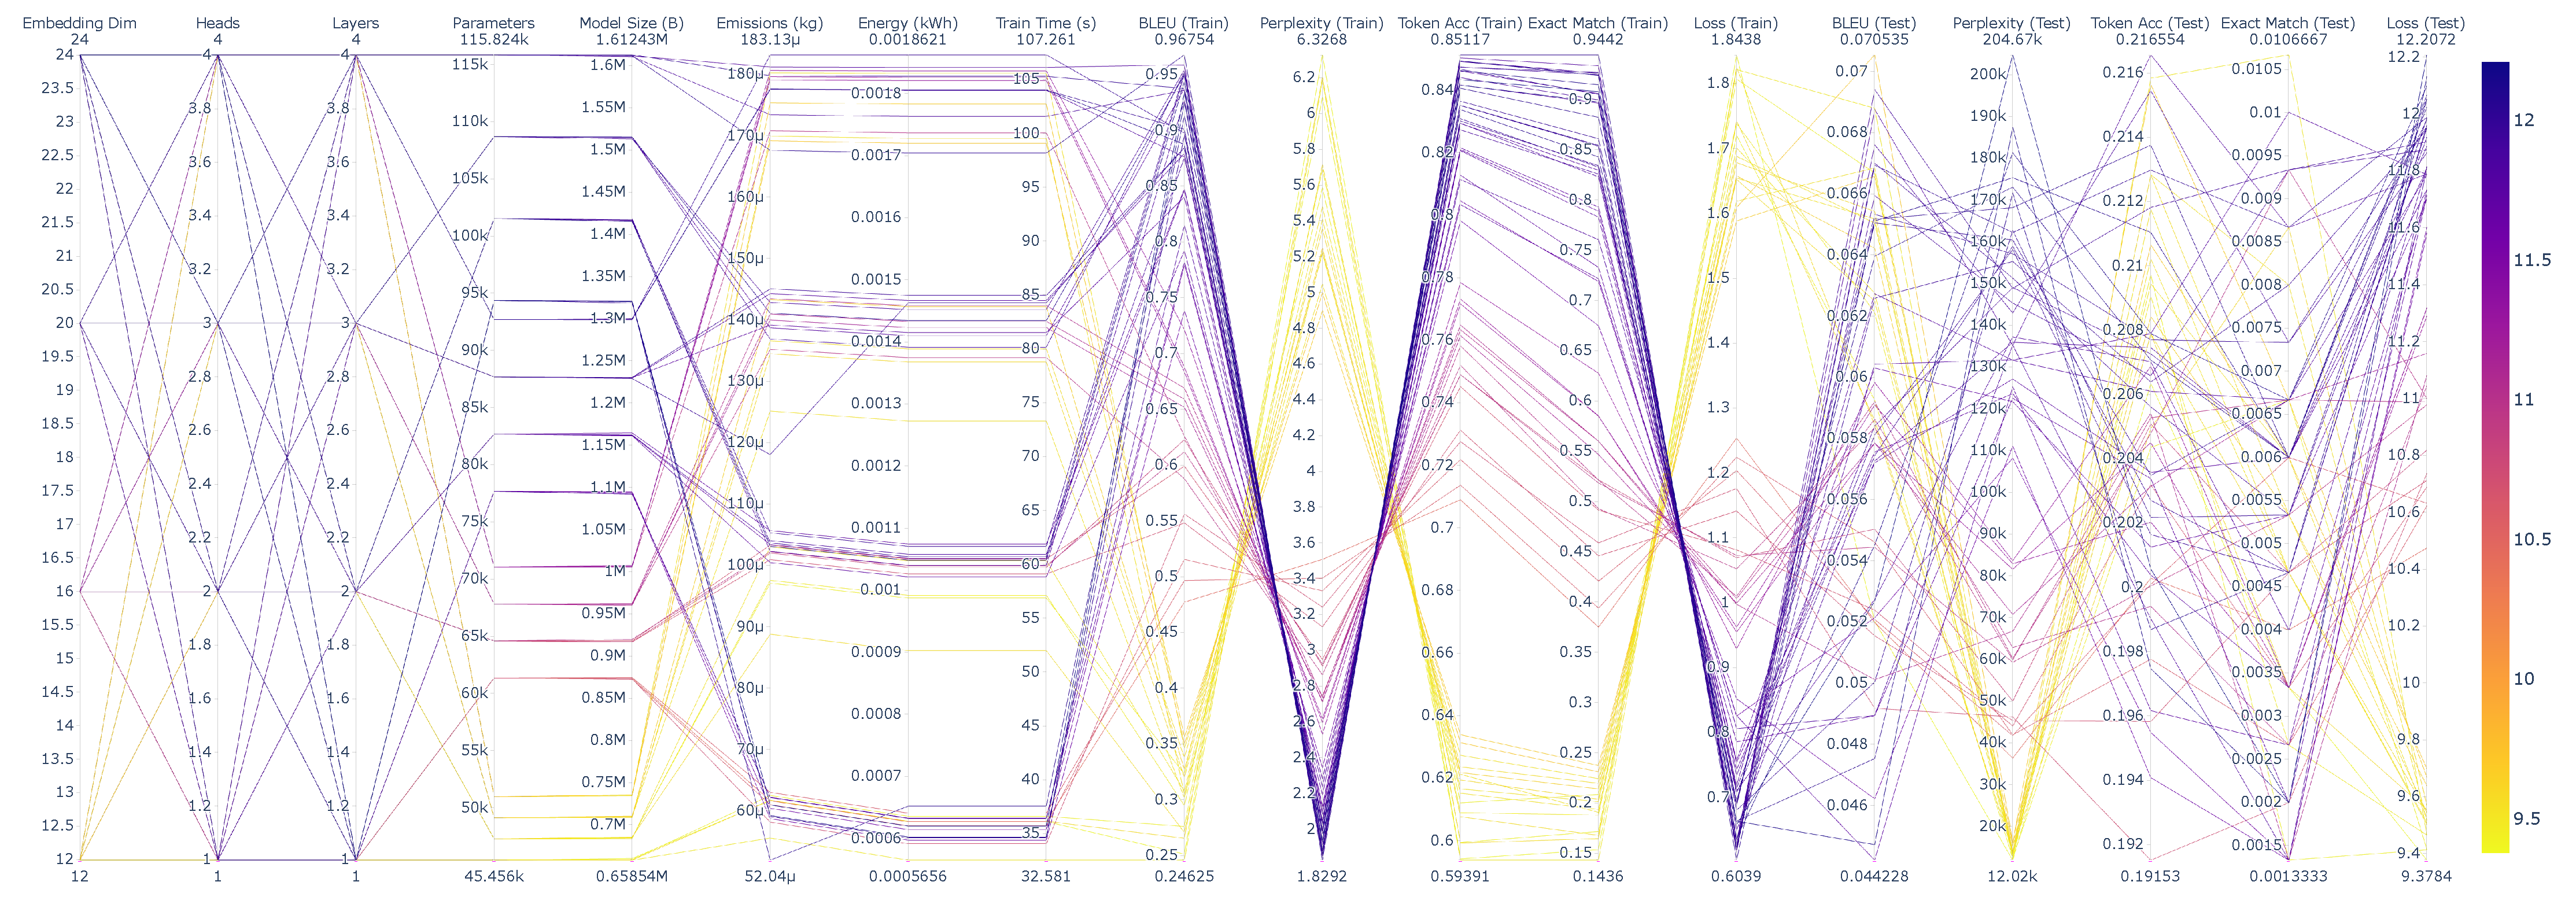
\includegraphics[
                width=\textheight,
                height=5\textwidth,
                keepaspectratio
            ]{Figures/parallel_result.pdf}
            \caption{Overview of FP32 baseline performance across architectural configurations. The results represent the mean of five independent runs. Increases in $d_{model}$, depth, and the number of heads improve training metrics but also amplify overfitting and computational cost.}
            \label{fig:parallel_coordinates}
        \end{minipage}
    }
\end{sidewaysfigure*}

\subsection{Safety-Oriented Quality Analysis}

Table~\ref{tab:safety_metrics} presents the four safety-oriented metrics evaluated separately on the training and test subsets, with results averaged over all combinations of $h \in \{1,2,3,4\}$ and $L \in \{1,2,3,4\}$ using five independent runs for each configuration. Overall, these results are consistent with the overfitting pattern observed with conventional metrics and provide an additional view of the safety behavior of the generated outputs.



\begin{table*}[htbp]
\small
\centering
\caption{Safety-oriented evaluation metrics for different embedding dimensions ($d_{\mathrm{model}}$). Values are reported as mean $\pm$ standard deviation over all combinations of $h\in\{1,2,3,4\}$, $L\in\{1,2,3,4\}$, and five independent runs. FC: Factual Correctness Rate; MG: Manual Grounding Score; HR: Hallucination Rate; UR: Unsafe Answer Rate.\\}
\label{tab:safety_metrics}
\begin{tabular}{clcccc}
\toprule
$d_\text{model}$ & Subset & FC (\%) & MG (\%) & HR (\%) & UR (\%) \\
\midrule
\multirow{2}{*}{12} & Train & $14.19 \pm 2.13$ & $32.99 \pm 3.48$ & $65.44 \pm 3.37$ & $0.186 \pm 0.049$ \\
                    & Test  & $0.41 \pm 0.20$  & $8.06 \pm 0.55$  & $91.14 \pm 0.70$ & $0.129 \pm 0.093$ \\
\midrule
\multirow{2}{*}{16} & Train & $42.77 \pm 7.61$ & $67.44 \pm 13.05$ & $31.64 \pm 12.71$ & $0.169 \pm 0.060$ \\
                    & Test  & $0.30 \pm 0.26$  & $6.35 \pm 1.10$   & $93.08 \pm 1.21$  & $0.138 \pm 0.110$ \\
\midrule
\multirow{2}{*}{20} & Train & $65.51 \pm 4.67$ & $85.48 \pm 4.81$ & $14.05 \pm 4.75$ & $0.196 \pm 0.022$ \\
                    & Test  & $0.46 \pm 0.22$  & $7.05 \pm 0.78$  & $92.37 \pm 0.94$ & $0.142 \pm 0.103$ \\
\midrule
\multirow{2}{*}{24} & Train & $75.44 \pm 1.74$ & $94.42 \pm 1.71$ & $5.38 \pm 1.63$  & $0.196 \pm 0.021$ \\
                    & Test  & $0.73 \pm 0.30$  & $7.49 \pm 0.96$  & $91.96 \pm 1.09$ & $0.108 \pm 0.073$ \\
\bottomrule
\end{tabular}
\end{table*}



On the training subset, all four metrics improve monotonically as $d_\text{model}$ increases. At $d_\text{model}=24$, the Factual Correctness Rate is $75.44\%\pm1.74\%$, the Manual Grounding Score is $94.42\%\pm1.71\%$, and the Hallucination Rate decreases to $5.38\%\pm1.63\%$, indicating that configurations with larger $d_\text{model}$ store the training corpus in their weight matrices with higher training-set alignment and produce outputs that more frequently match the reference answers. In contrast, at $d_\text{model}=12$, the Factual Correctness Rate is $14.19\%\pm2.13\%$, and the Hallucination Rate is $65.44\%\pm3.37\%$, which suggests that this setting has limited capacity to memorize the training data. The individual configuration $h=4$, $L=4$, $d_\text{model}=24$ achieves a Factual Correctness Rate of $78.16\%$, a Manual Grounding Score of $96.98\%$, and a Hallucination Rate of $3.00\%$.


On the test subset, the results show a different pattern, with Factual Correctness remaining below $1.1\%$ for all configurations, Manual Grounding scores ranging from $6.35\%$ to $8.06\%$, and the Hallucination Rate exceeding $91\%$ for every value of $d_\text{model}$. The lack of a capacity-dependent trend on the test set is consistent with the intentional overfitting design, since the model was not trained to generalize to unseen query phrasings. Instead, it acts as a closed parametric index of the training corpus, reproducing memorized entries while generating ungrounded outputs for queries outside the training distribution. This behavior matches the intended use of the model as a deterministic, offline retrieval mechanism for domain-specific knowledge stored in a compact weight representation.


The Unsafe Answer Rate remains low across all configurations and both subsets. On the test set, the mean Unsafe Answer Rate is $0.129\%$, with a maximum value of $0.400\%$ across all 64 evaluated configurations, while on the training set the rate remains below $0.200\%$. These results suggest that, when the model fails to retrieve a memorized pattern, it usually generates incomplete or degenerate token sequences rather than factually incorrect safety instructions. This behavior is consistent with the low-capacity, closed-vocabulary design, which limits the model's ability to produce coherent false claims. In this work, out-of-distribution inputs therefore tend to produce empty or truncated responses rather than incorrect guidance, which is a safer failure mode for automotive applications, particularly when the query involves safety-related vehicle information.



\subsection{Hardware-Aware Performance Analysis}
\label{subsec:hardware_eval}

Figure~\ref{fig:hardware_performance} presents model deployment across Portenta H7, ESP32, Pi Pico, and Nano 33 BLE microcontrollers for configurations with embedding dimension $d_{model}=24,20,16,12$, $h=4$, and $L=4$. Flash memory usage ranges from 315824 B to 782206 B. RAM consumption spans 34060 B to 81824 B. Inference time varies from 0.0934 s to 23.2131 s. Energy consumption ranges from 84.59 mW to 366.73 mW.

\begin{figure}[htbp]
    \centering
    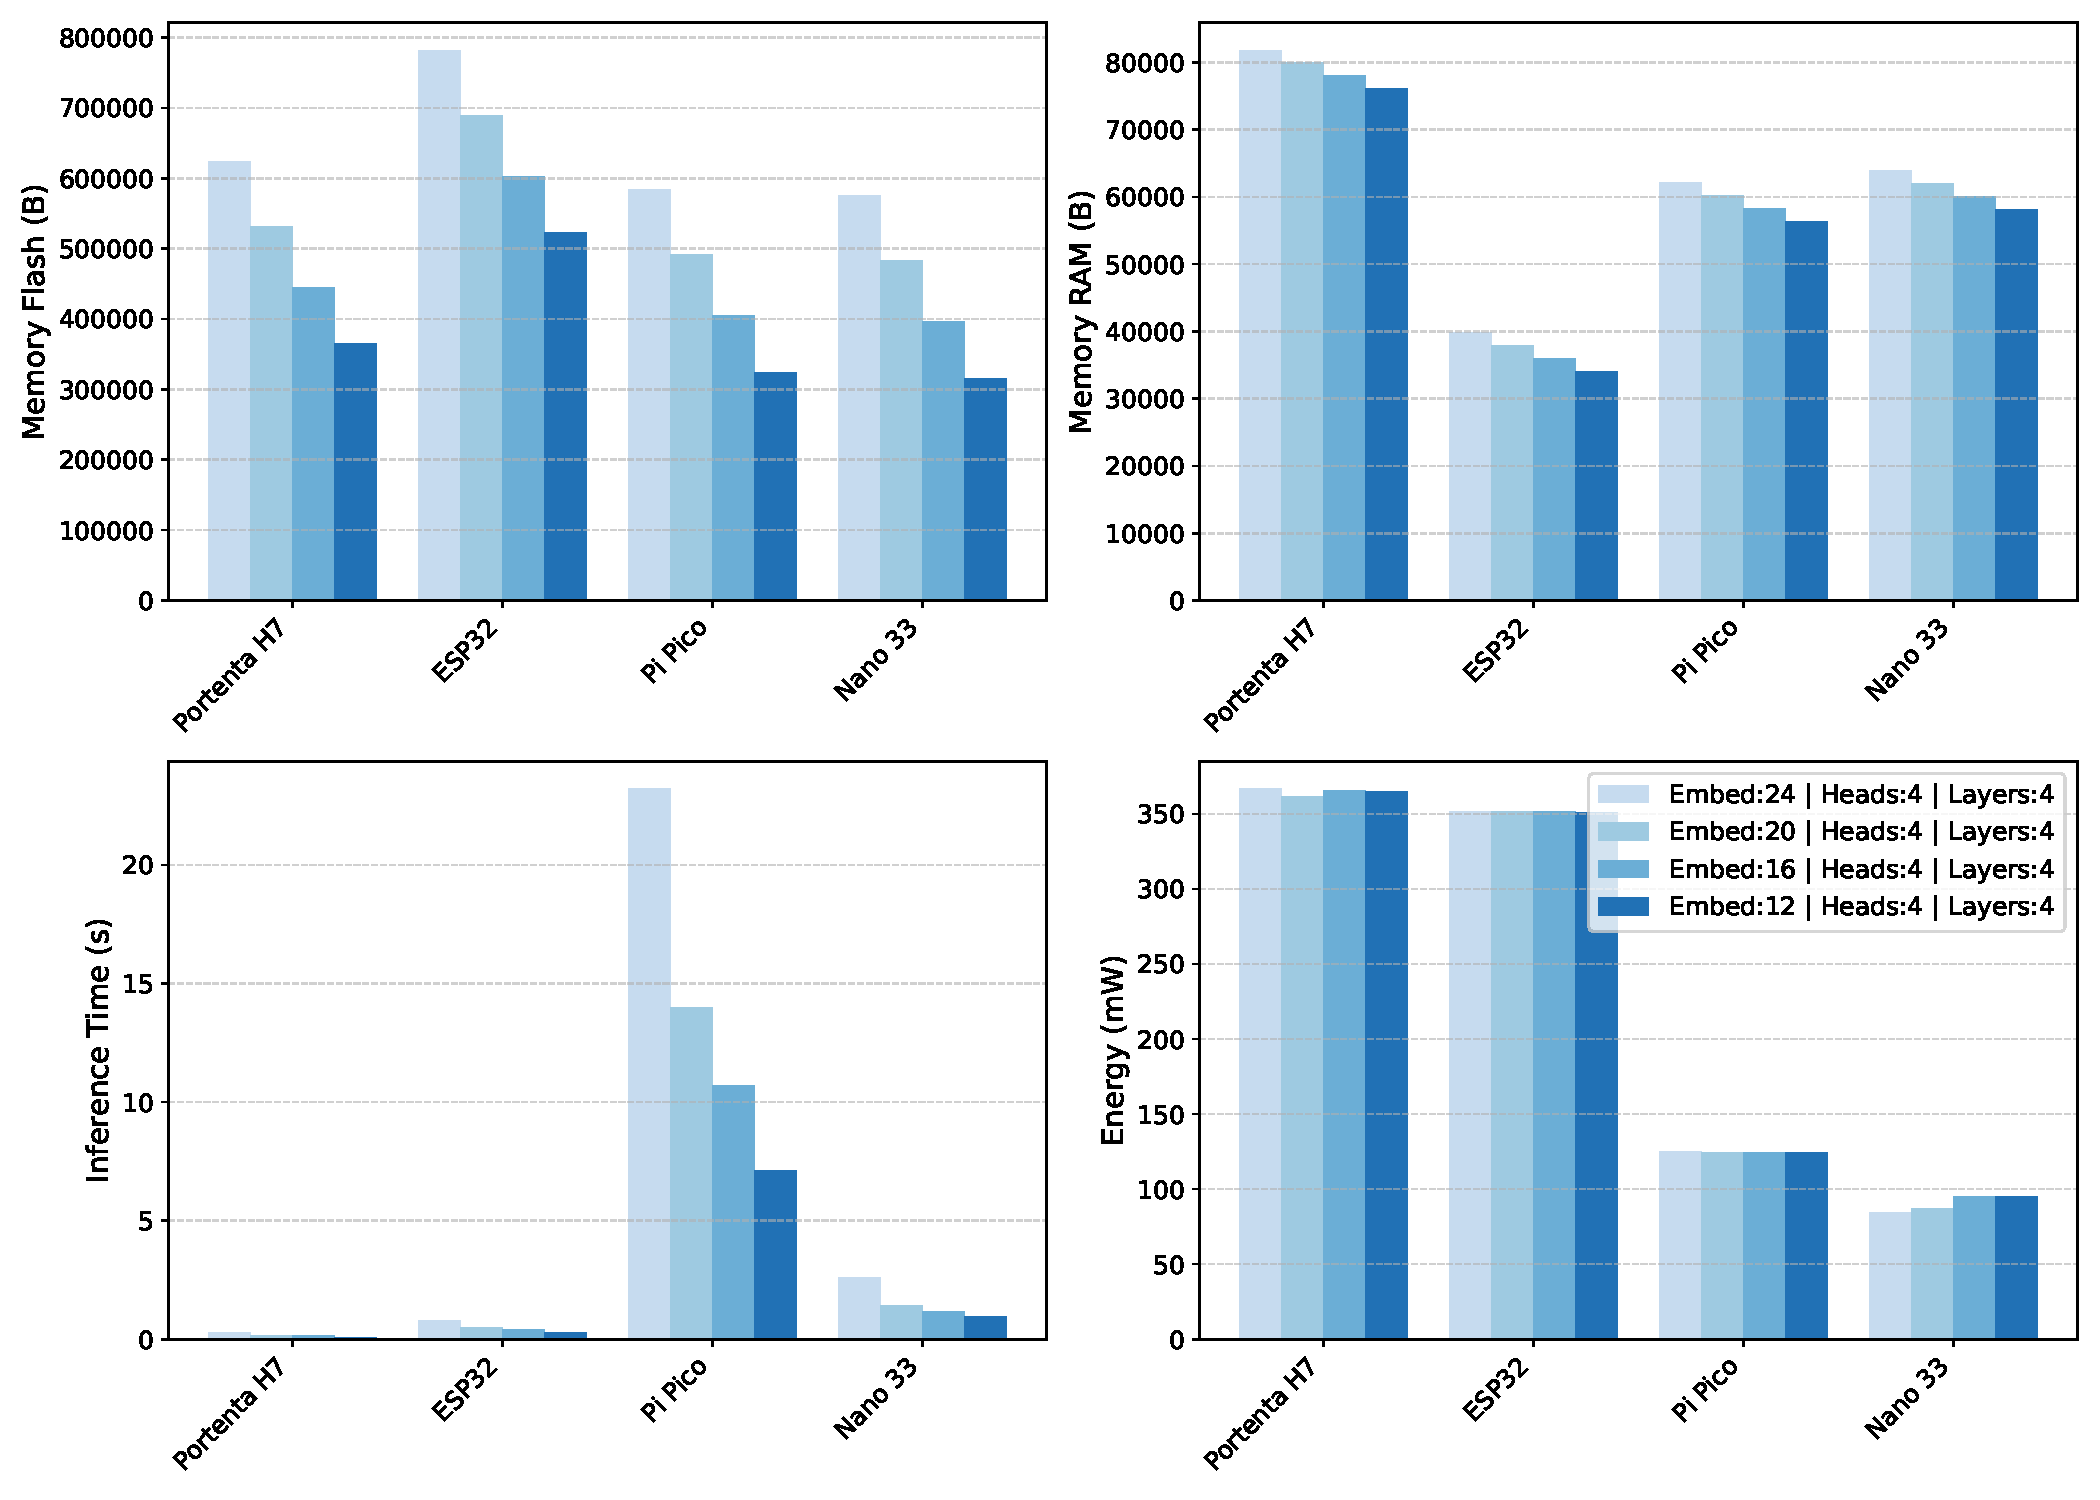
\includegraphics[width=1\linewidth]{Figures/hardware_performance_barplots_2x2.pdf}
    \caption{Hardware performance across Portenta H7, ESP32, Pi Pico, and Nano 33 BLE evaluating Flash memory, RAM usage, inference time, and energy consumption for $d_{model}=24,20,16,12$ with $h=4$, $L=4$.}
    \label{fig:hardware_performance}
\end{figure}



Portenta H7 records inference times below 0.3 s across all configurations due to Cortex-M7 architecture at 480 MHz with hardware FPU and DSP extensions. ESP32 inference times remain below 0.9 s through Xtensa LX6 dual-core processing. Pi Pico requires 7.13 s to 23.21 s because the Cortex-M0+ core lacks a hardware FPU and must execute floating-point matrix operations in software at 133 MHz; these latencies are too high for interactive use cases and highlight that the proposed approach is not suitable for real-time deployment on integer-only microcontrollers without further quantization. Nano 33 BLE maintains inference below 2.6 s through Cortex-M4F single-cycle MAC instructions despite 64 MHz clock.

Flash memory consumption correlates with compiler backend and instruction set encoding. ESP32 requires flash storage exceeding 700 kB across configurations due to Xtensa code density requirements. Portenta H7 and Nano 33 BLE ARM toolchains produce smaller binaries below 650 kB. RAM usage follows static allocation patterns determined by activation maps and attention buffers. ESP32 minimizes RAM usage below 40 kB by using stack-based temporary storage. Portenta H7 allocates more than 75 kB of memory for larger activation buffers aligned to cache line boundaries.

Energy profiles reflect core voltage and peripheral activation during inference. Portenta H7 consumes 350-367 mW through sustained high-frequency operation. Nano 33 BLE and Pi Pico operate below 125 mW with sleep-state transitions between tensor operations. ESP32 maintains an average of 350 mW despite dynamic frequency scaling. Inference time dominates energy proportionality across boards, since matrix multiplications account for over 95\% of Transformer floating-point operations.

All deployments execute natively in C++ with identical tensor implementations across platforms. Source-level portability eliminates vendor-specific intrinsics or runtime dependencies. Deterministic execution enables reproducible latency measurements across hardware generations and compiler versions.




\subsection{Comparative Positioning within the Edge AI Landscape}

To rigorously contextualize the performance of Extreme TinyGPT, we benchmarked our approach against state-of-the-art frameworks identified in the literature. The Transformers-on-microcontrollers landscape is primarily divided into discriminative models, which operate as encoders, and generative models, which function as decoders, each exhibiting distinct computational and memory profiles.

Discriminative and vision-oriented baselines, such as MCUBERT \cite{10.1145/3676536.3676747} and TinyFormer \cite{yang2023tinyformer}, have demonstrated the feasibility of deploying encoder-only architectures on generic microcontrollers. These approaches are optimized for classification-centric tasks, including intent detection and gesture recognition, rather than autoregressive text generation. Similarly, MCUFormer \cite{liang2023mcuformer} extends Transformer-based inference to computer vision by deploying Vision Transformers on STM32 devices using One-Shot Neural Architecture Search (NAS) to satisfy memory constraints. While these models achieve high efficiency and often fit within sub-500\,KB Flash budgets, they do not address the Key-Value cache management and sequential dependency inherent to generative Question-Answering tasks.

Within the generative domain, Deeploy \cite{scherer2024deeploy} represents the closest functional counterpart, enabling the execution of Small Language Models on heterogeneous microcontrollers through NPU acceleration. Beyond bare-metal MCUs, recent studies have explored Embedded LLMs for enhanced Human–Machine Interfaces in autonomous vehicles \cite{varshni2025embedded} and for integrating generative language models into IoT devices \cite{yauri2024generative}. Although these works validate the utility of generative interaction in automotive and smart-home contexts, they typically rely on high-performance edge computers or Linux-based SoCs to meet the memory and compute demands of larger models.

While a performance gap exists between Extreme TinyGPT and billion-parameter models, such as TinyLlama-1.1B, this difference must be interpreted within the operational envelope. Models at the billion-parameter scale require gigabytes of memory and dedicated NPUs or GPUs, making their execution infeasible on the microcontrollers considered here. In contrast, Extreme TinyGPT targets a different design point, enabling parametric text generation on resource-constrained, sub-watt hardware. This configuration favors offline execution, deterministic implementation, and deployment on low-cost devices, while limiting out-of-distribution QA quality compared with larger models or retrieval-based systems.



As illustrated in Figure~\ref{fig:tinygpt_landscape}, Extreme TinyGPT occupies a specific position by providing a generative, floating-point, deterministic, and dependency-free implementation on standard Cortex-M and Xtensa architectures without specialized hardware support. Although it incurs higher latency than accelerated solutions and does not retain a retrieval component at inference time, it characterizes the design space between encoder-only classification systems and high-end edge generative platforms. The resulting implementation supports software-level auditability for safety-aware experimentation.

Lightweight retrieval alternatives, including keyword search, BM25, vector retrieval, and answer lookup, remain reference points for vehicle-manual QA. These methods can provide document grounding when the manual or an index is available at inference time, whereas Extreme TinyGPT explores a different design point in which selected manual knowledge is encoded within FP32 weights and no document store is retained on the MCU. This choice reduces runtime dependencies and storage requirements while limiting out-of-distribution factual coverage. A systematic comparison with retrieval and lookup baselines is therefore left as future work.


\begin{figure}[htpb]
    \centering
    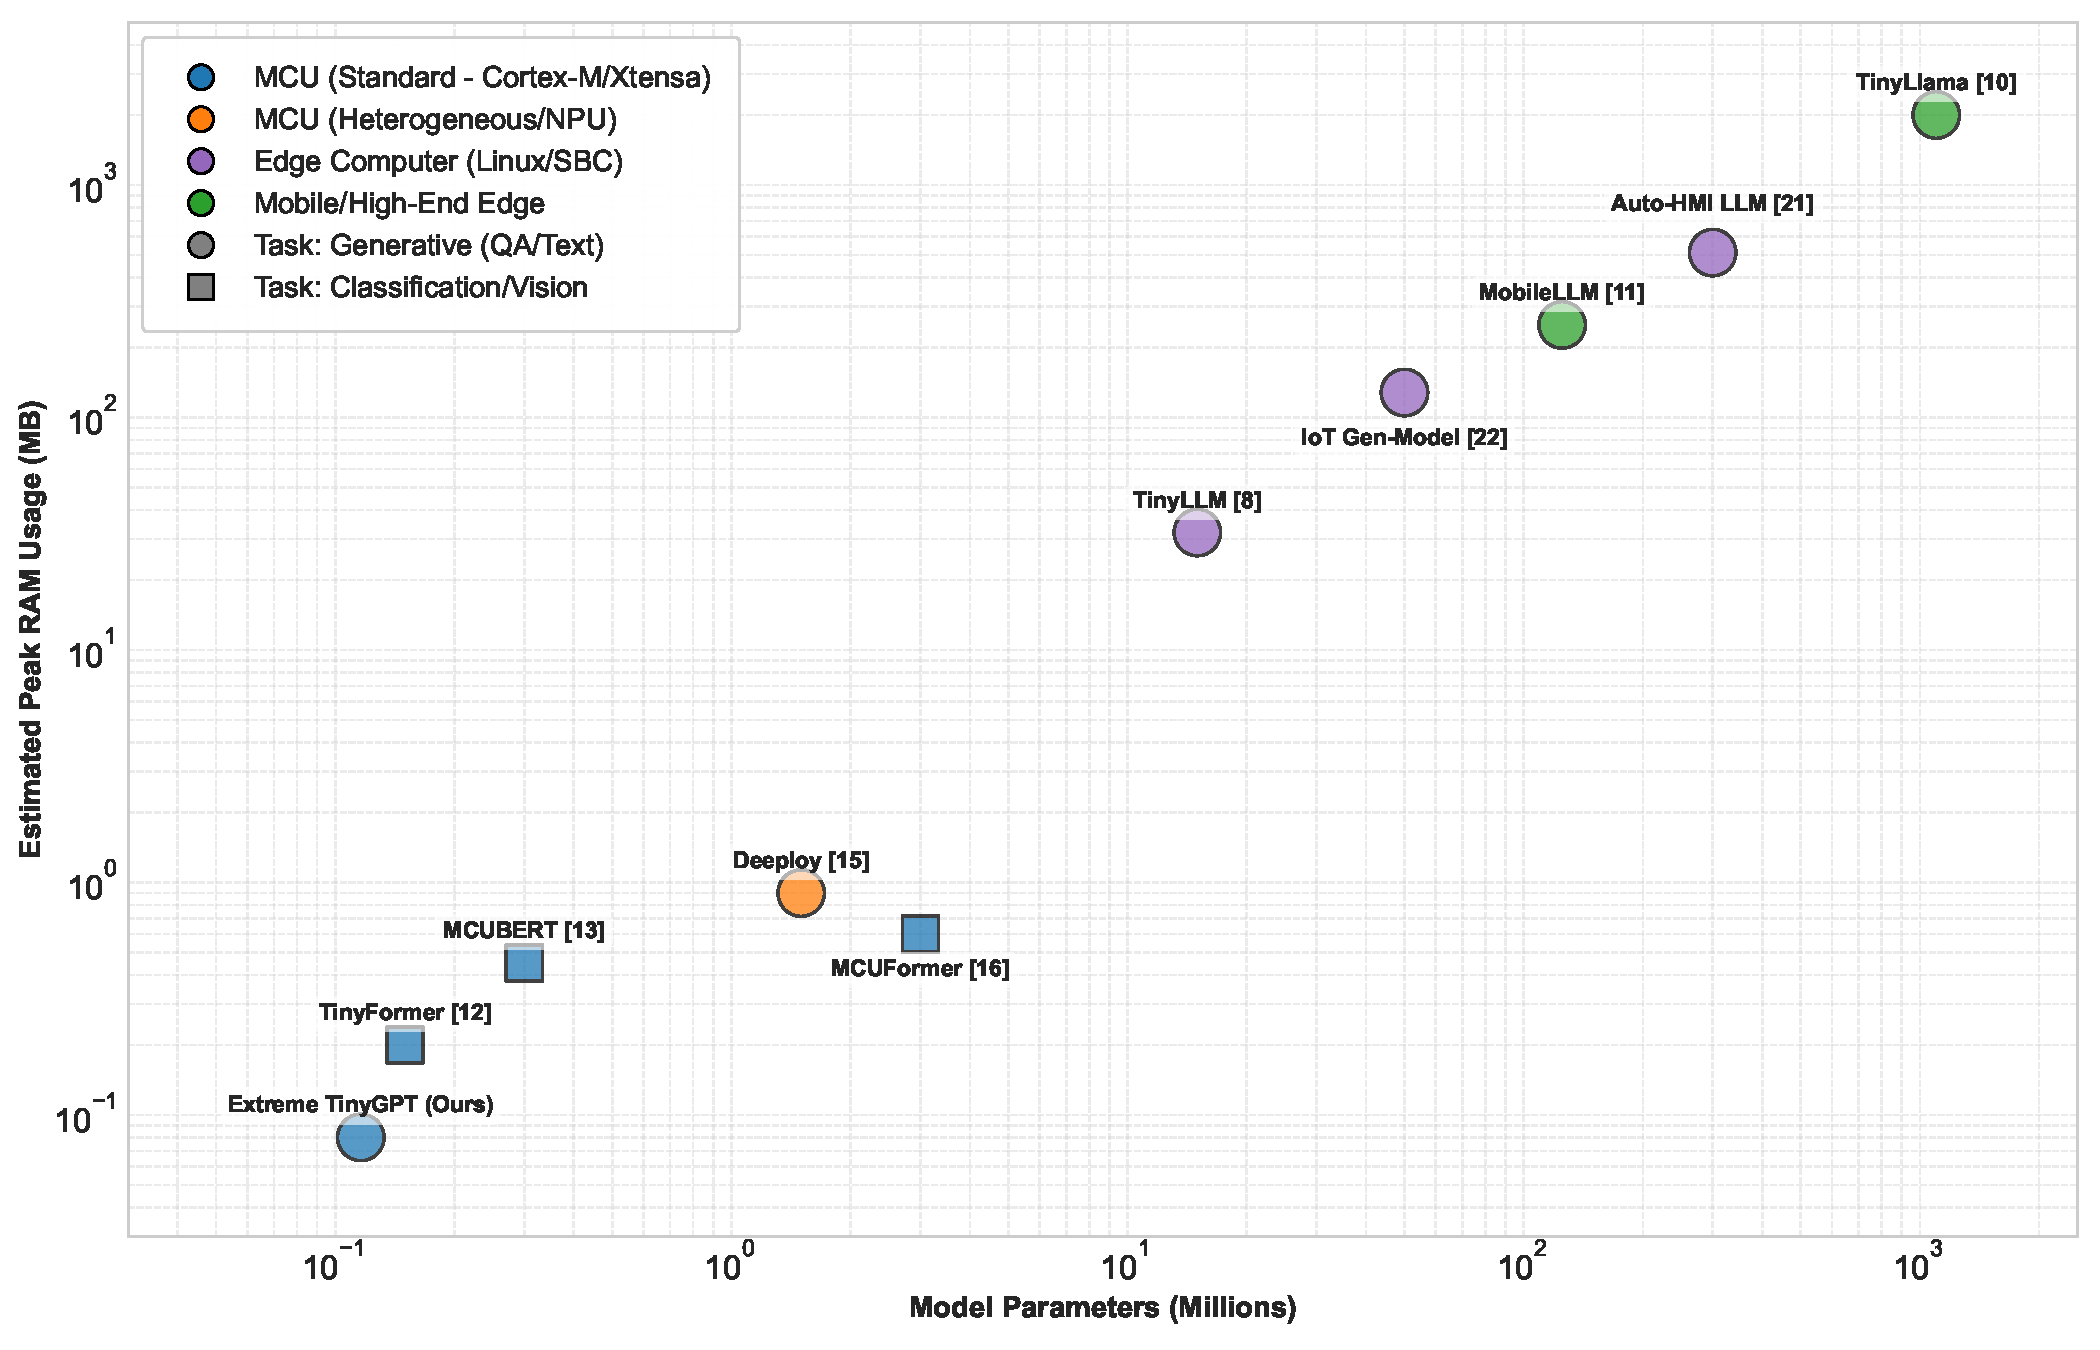
\includegraphics[width=1\linewidth]{Figures/tinygpt_landscape_final.pdf}
    \caption{Comparative landscape of State-of-the-Art EdgeAI models. The chart plots model complexity (number of parameters) against estimated peak RAM usage on a logarithmic scale. Data points are color-coded by hardware target and shaped by primary task (circles for generative, squares for discriminative). Extreme TinyGPT occupies a specific position, enabling generative capabilities on standard microcontrollers (Cortex-M, Xtensa) with a small resource footprint, compared with classifier-focused MCU models (MCUBERT) and hardware-accelerated generative frameworks (Deeploy).}
    \label{fig:tinygpt_landscape}
\end{figure}




\section{Conclusion}\label{sec:conclusion}

This work introduced Extreme TinyGPT as a specialized framework for deploying a compact parametric generative model on resource-constrained embedded systems. Offline RAG is used to generate synthetic question-answer pairs, which are then compressed into the model's weights for retrieval-free MCU inference. Through transparent parameter export and a streamlined Python-to-C++ conversion pipeline, the proposed methodology enables offline and auditable inference on bare-metal microcontrollers. This capability is relevant to automotive applications where independent execution, code traceability, and low-cost deployment are design requirements.

The results lead to three main conclusions. First, unlike discriminative baselines such as MCUBERT, which are limited to classification, the proposed approach enables autoregressive generation on standard microcontroller architectures such as Cortex-M and Xtensa. Second, unlike generative deployment frameworks that rely on Neural Processing Units or opaque vendor-specific compilers, including Deeploy, the proposed implementation remains inspectable. The preservation of 32-bit floating-point precision supports deterministic execution and source-level inspection, while answer quality is assessed separately through predictive and safety-oriented metrics. Third, the experimental results show millisecond-level latency on FPU-enabled devices such as the Portenta H7 and sub-watt operation on platforms such as the Arduino Nano 33 BLE, with higher latency observed on lower-end integer-oriented devices.

These contributions involve trade-offs. In terms of predictive accuracy, the proposed model remains below Linux-class models such as TinyLlama-1.1B, as expected given the kilobyte-scale memory constraints of microcontroller platforms. The test BLEU, perplexity, exact-match, and loss values indicate that generalization to unseen formulations remains limited, even though the model can execute on MCU-class hardware and encode the training domain. The results also show that inference efficiency depends on hardware Floating Point Units, with performance degradation on integer-only architectures such as the Raspberry Pi Pico. Accordingly, the proposed model can be viewed as a constrained embedded deployment strategy for settings in which power efficiency, cost, transparency, and auditability take precedence over general linguistic coverage.

In automotive settings, environmental conditions impose additional constraints on on-device inference. Thermal effects can influence both reliability and performance in embedded platforms. Prior work on microcontrollers with AI accelerators has shown that elevated operating temperatures can reduce device lifetime and trigger thermal throttling, which may degrade quality of service during sustained inference workloads~\cite{10.1145/3662009.3662020} \cite{electronics13112012}. Reliability studies have also reported temperature-dependent soft-error rates in embedded SRAM, with greater susceptibility at elevated temperatures. A thermal characterization of the proposed MCU deployment is therefore a direction for future work, although it remains outside the primary scope of the present study.

The safety-oriented evaluation is consistent with the intended closed-domain behavior of the proposed model. On the training set, the configuration with the largest evaluated capacity ($h=4$, $L=4$, $d_\text{model}=24$) achieves a Factual Correctness Rate of $78.16\%$, a Manual Grounding Score of $96.98\%$, and a Hallucination Rate of $3.00\%$, indicating that the model can encode the target domain within its FP32 weight matrices. On the test set, Factual Correctness remains below $1.1\%$ and the Hallucination Rate exceeds $90\%$ for every evaluated configuration, showing that the model does not generalize to unseen query formulations. This behavior is consistent with the design objective, which favors deterministic reproduction of memorized domain knowledge rather than open-ended generalization.

The Unsafe Answer Rate is below $0.40\%$ across all configurations and both subsets, with a test-set mean of $0.13\%$. In this work, out-of-distribution inputs generally produce incomplete or degenerate outputs rather than unsafe guidance. This failure mode is preferable for automotive applications, where an empty or truncated response is less risky than an incorrect safety-related instruction. Future work should extend factual coverage while preserving this behavior, with emphasis on retrieval-augmented inference at the MCU level, quantization-aware training to reduce FPU dependence, dataset expansion, and integration with vehicle diagnostics through OBD-II. These directions may extend domain coverage while supporting consistent evaluation protocols for probabilistic NLP in embedded systems.



\bibliographystyle{ieeetr}
\bibliography{references}

\vspace*{-1.0cm}

\begin{IEEEbiography}[{
\includegraphics[width=1in,height=1.25in,clip,keepaspectratio]{author1.jpg}}]{Thommas K. S. Flores} is an Assistant Professor with the Department of Computing and Technology, Federal University of Rio Grande do Norte (UFRN), Brazil. He received the B.S. and M.S. degrees in Electrical Engineering from the Federal University of Paraíba (UFPB), Brazil, in 2018 and 2021, respectively, and the Ph.D. degree in Electrical and Computer Engineering from UFRN in 2026. His research interests include TinyML, Edge AI, intelligent embedded systems, evolutionary quantization of large language models, and MLOps for the Internet of Intelligent Vehicles and advanced manufacturing. He is the author of the Extreme TinyGPT and TensorFlores frameworks.
\end{IEEEbiography}

\vspace*{-1.0cm}

\begin{IEEEbiography}[{
\includegraphics[width=1in,height=1.25in,clip,keepaspectratio]{author2.jpg}}]{Daniel G. Costa (Senior Member, IEEE)} is an Assistant Professor of the Department of Electrical and Computer Engineering (DEEC), Faculty of Engineering (FEUP), University of Porto. He is an author or co-author of more than 100 international scientific papers in prestigious journals and conferences, covering research topics in the areas of Smart Cities, Internet of Things, Sensor Networks, Embedded Systems and Multimedia Sensing.
\end{IEEEbiography}

\vspace*{-1.0cm}

\begin{IEEEbiography}[{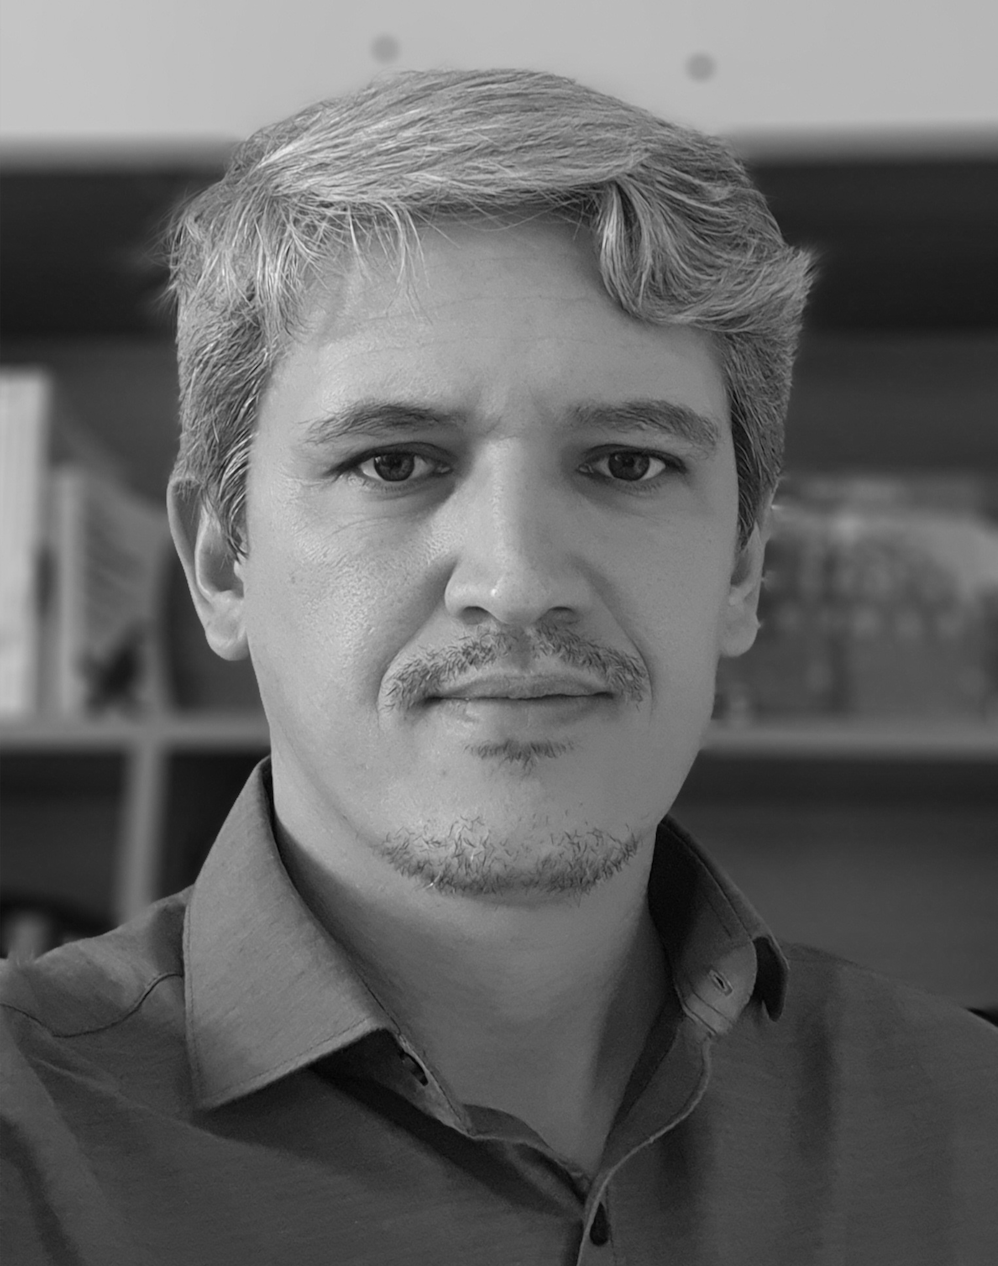
\includegraphics[width=1in,height=1.25in,clip,keepaspectratio]{author3.png}}]{Ivanovitch Silva (Senior Member, IEEE)} earned his B.S. (2006), M.Sc. (2008), and Ph.D. (2013) degrees in Electrical and Computer Engineering from the Federal University of Rio Grande do Norte (UFRN), Brazil, with a co-participation from the University of Porto Portugal. Currently, he is an Associate Professor at UFRN's Department of Computer Engineering and Automation (DCA), and in 2021, he served as a Visiting Professor at the Università degli Studi di Brescia, Italy.  His research interests focus on Embedded AI, MLOps, Internet of Intelligent Vehicles and Sustainable Cities.
\end{IEEEbiography}





\EOD

\end{document}
